\chapter{Semantica Computazionale}

\section{Introduzione}

\subsection{Semantica Computazionale}

\paragraph{La semantica computazionale (fig: \ref{fig:sem}) può essere divisa grossolonamente in tre parti:}

\begin{itemize}
  \item \fancyglitter{Semantica lessicale:} consiste nello studio di \textit{come} e \textit{che cosa} denotano le parole di una lingua. Si analizzano:
    \begin{itemize}
      \item \evidence{Significato letterale}. 
      \item \evidence{Polisemia:} parole con più significati.
      \item \evidence{Relazioni semantiche:} sinonimia, antonimia, iponimia, etc. 
      \item \evidence{Composizione del significato}.
    \end{itemize}
  \item \fancyglitter{Semantica formale:} studia i modelli logico-matematici che definiscono formalmente i linguaggi. L'obiettivo è definire il significato in termini di condizioni di verità.
  \item \fancyglitter{Semantica statistico-distribuzionale:} approccio computazionale e quantitativo al significato che combina metodi statistici e intuizioni linguistiche (in particolare il fatto che il significato delle parole possa essere inferito dalla loro distribuzione sui testi). Si analizzano grandi corpora per costruire rappresentazioni vettoriali delle parole (\textit{embeddings}), in cui la vicinanza tra vettori (solitamente si usa la \textit{cosine similarity}) riflette la somigliarità semantica. 

\end{itemize}

\begin{figure}[h]
    \centering
    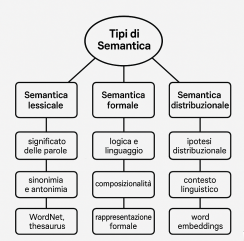
\includegraphics[scale=0.6]{01/sem.png}
    \caption{Tipi di semantica.}
    \label{fig:sem}

  \end{figure}

\subsection{Origini del NLP}

Inizialmente la linguistica computazionale e l'elaborazione del linguaggio naturale si occupavano del \fancyglitter{question answering} (Q\&A) ossia permettere a una macchina di leggere un testo (\textit{what}) e rispondere a domande poste da un utente (\textit{why}) attraverso l'impiego di codice e di risorse linguistiche (\textit{how}). Con il passare del tempo le domande sono diventate sempre più complesse e variegate riguardando: fatti specifici, richieste di elenchi, definizioni, motivazioni, elenchi, etc.  

Proprio per questo motivo è emersa una nuova area di ricerca appositamente per la caratterizzazione delle domande. L'obiettivo è quello di costruire tassonomie per modellare ogni possibile sfaccettatura che una domanda possa avere. Tutto ciò per aumentare l'efficacia dei sistemi di Q\&A che necessitano, in primo luogo, di comprendere la tipologia di domanda. 

Negli ultimi, grazie allo sviluppo dell'\fancyglitter{intelligenza artificiale generativa} (e dei modelli GPT, LLaMA, etc.), il Q\&A si è evoluto. Questi modelli possono estrarre domande da un testo e \textit{generare} risposte articolate, sintetiche o creative. Possono:
\begin{itemize}
  \item Rispondere a domande complesse. 
  \item Gestire dialoghi multi turno. 
  \item Tradurre le domande e le risposte. 
  \item Spiegare le proprie risposte.
\end{itemize}

\nt{Quindi è ancora più importante determinare il contenuto della domanda in modo da evitare \fancyglitter{allucinazioni}.
Storicamente il Q\&A è sempre stato un task complesso, ma nel periodo post-ChatGPT sta vedendo il suo apice mediante il meccanismo chiamato \fancyglitter{prompting}.}

Gran parte della ricerca non si limita al Q\&A, ma anche a ciò che ci sta dietro o in parallelo. Per esempio PoS, NeR tagging, iperonimi, word sense disambiguation, etc.  Oppure casi come quello del \textit{suggeritore automatico}, presente nelle tastiere degli smartphone, che usa un modello statistico.


\subsection{Word Sense Induction}

\dfn{Word Sense Induction}{
  La Word Sense Induction (WSI) è il task che riguarda l'identificazione del senso di una parola polisemica in una frase, all'interno di un determinato contesto.
}

\paragraph{Questo task ha problemi di:}

\begin{itemize}
  \item \fancyglitter{Specificità:} molti sensi attribuiti alle parole non vengono utilizzati perché troppo specifici e sono solamente \textit{rumore}. Questo è criticato da vari studiosi che sostengono sia necessario aggregare alcuni sensi troppo simili (e.g. in WordNet). 
  \item \fancyglitter{Copertura:} ci sono molte zone di linguaggio non coperte. 
  \item \fancyglitter{Soggettività:} nonostante le decisioni siano prese collettivamente c'è  sempre una componente soggettiva.
\end{itemize}

\paragraph{Differenze tra Word Sense Induction (WSI) e Word Sense Disambiguation (WSD):}

\begin{itemize}
  \item La disambiguazione ha necessità di un dizionario/sense inventory (e.g. WordNet) che contiene tutti i possibili sensi per ogni parola. Nel WSI non esiste un dizionario. 
  \item Nel WSI ci si basa sull'effettivo uso della parola in grandi quantità di dati.  
  \item La WSD, essendo fatta da linguisti, è basata sulla grammatica. La WSI è basata sull'uso delle parole, anche sgrammaticato. 
  \item La valutazionw nel WSD è semplice (per esempio usando synsets gold), ma criticabile come visto in precedenza. Nel WSI è un po' più complicato.
\end{itemize}

\cor{Pseudo-word}{
  Il metodo della Pseudo-word è una tecnica per valutare algoritmi di WSI in assenza di risorse semantiche o annotazioni di senso. L'idea è quella di simulare l'ambiguità lessicale creando artificialmente delle parole ambigue e poi testare se il sistema è in grado di distinguerne i sensi sottostanti.
}

\paragraph{Fasi della Pseudo-word:}

\begin{enumerate}
  \item \fancyglitter{Merging:} concatenazione di parole reali. Consiste nel fondere due o più parole esistenti in una parola ambigua. Queste parole devono avere significati distinti e usi in contesti diversi.
  \item \fancyglitter{Substitution:} sostituzione nei contesti. Tutte le occorrenze delle parole originali vengono sostituite nei testi dalla nuova parola create nel merging.
  \item \fancyglitter{Clustering:} identificazione dei sensi. Si applica un algoritmo di clustering (e.g. k-means, DB-SCAN, o modelli basati su embeddings) sulle rappresentazioni contestuali delle Pseudo-word per scoprire gruppi di usi distinti (sensi). 
  \item \fancyglitter{Cluster-to-Class evaluation:} valutazione. Si valuta la qualità dei clusters ottenuti confrontandoli con le parole originali 
\end{enumerate}

\paragraph{Vantaggi e Limiti:}

\begin{itemize}
  \item [\textcolor{green}{\ding{51}}] Non sono richieste annotazioni manuali o risorse linguistiche.
      \item [\textcolor{green}{\ding{51}}] Può essere usato su grandi corpora in maniera automatica.
  \item [\textcolor{red}{\ding{55}}] I sensi creati non riflettono ambiguità reali. 
  \item [\textcolor{red}{\ding{55}}] I contesti potrebbero essere troppo distinti e causare \textit{overfitting}. 
\end{itemize}

\subsection{Comprensione del Linguaggio Naturale}

\begin{itemize}
  \item \fancyglitter{Dizionari Elettronici:}
    \begin{itemize}
      \item \evidence{Potere espressivo:} medio-alto, forniscono relazioni semantiche ricche. 
      \item \evidence{Scalabilità:} medio-bassa, solitamente sono costruiti manualmente (quindi difficilmente estendibili).
      \item \evidence{Sorgente:} curata manualmente da esperti linguisti.
      \item \evidence{Ambiguità e Soggettività:} ambiguità ridotta, soggettività media (su accezioni meno comuni).
    \end{itemize}
  \item \fancyglitter{Property Norms:}
    \begin{itemize}
      \item \evidence{Potere espressivo:} alto per concetti concreti.
      \item \evidence{Scalabilità:} bassa perché richiede raccolta tramite esperimenti psicologici o annotazioni.
      \item \evidence{Sorgente:} spesso da studi cognitivi o crowd-sourcing/mechanical turk.
      \item \evidence{Ambiguità e Soggettività:} alta, perché le persone non sono linguisti.
    \end{itemize}
  \item \fancyglitter{Frames:}
    \begin{itemize}
      \item \evidence{Potere espressivo:} alto, cattura le strutture sintattico-semantiche. 
      \item \evidence{Scalabilità:} media, possono essere ampliati con annotazioni automatiche, ma richiede risorse linguistiche robuste.
      \item \evidence{Sorgente:} tipicamente linguistica, contributi da annotatori esperti. 
      \item \evidence{Ambiguità e Soggettività:} media, perché c'è spesso intervento umano, ma si rimedia con strumenti automatici.
    \end{itemize}
  \item \fancyglitter{Senso Comune:}
    \begin{itemize}
      \item \evidence{Potere espressivo:} molto alto, copre inferenze, aspettative sociali e causalità.
      \item \evidence{Scalabilità:} media, dato che servono molte persone. 
      \item \evidence{Sorgente:} crowd-sourcing, scraping, machine learning.
      \item \evidence{Ambiguità e Soggettività:} molto alta, molte conoscenze sono implicite, culturali o controverse.
    \end{itemize}
    \item \fancyglitter{Visual Attributes:}
    \begin{itemize}
      \item \evidence{Potere espressivo:} medio, utile per oggetti visibili, ma limitato ad aspetti percettibili. 
      \item \evidence{Scalabilità:}  medio-alta con dataset di immagini annotate.
      \item \evidence{Sorgente:} dati visivi + annotazioni.
      \item \evidence{Ambiguità e Soggettività:} medio-alta, le percezioni visive sono soggettive.
    \end{itemize}
\item \fancyglitter{Word Embedding:}
    \begin{itemize}
      \item \evidence{Potere espressivo:} molto alto in contesti distribuzionali. 
      \item \evidence{Scalabilità:} molto alta, addestrabili su grandi corpora.
      \item \evidence{Sorgente:} dati testuali in grande scala.
      \item \evidence{Ambiguità e Soggettività:} medio-alta, dipendono dal contesto, dalla lingua e possono riflettere eventuali bias.
    \end{itemize}
\item \fancyglitter{Corpus Manager:}
    \begin{itemize}
      \item \evidence{Potere espressivo:} dipende dal corpus, utile per esplorare usi reali del linguaggio. 
      \item \evidence{Scalabilità:} alta, può gestire ilioni/miliardi di parole.
      \item \evidence{Sorgente:} testi reali.
      \item \evidence{Ambiguità e Soggettività:} media, i dati sono "grezzi", quindi l'ambiguità linguistica è intrinseca.
    \end{itemize}

\end{itemize}

\begin{figure}[h]
    \centering
    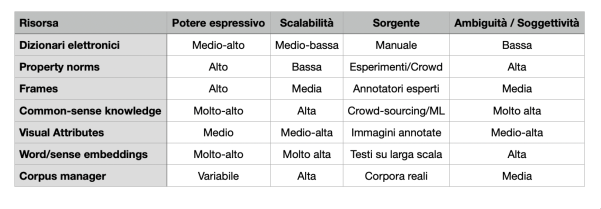
\includegraphics[scale=0.6]{01/riassunto.png}
    \caption{Schema delle risorse.}
\end{figure}

\section{Definizioni e Ricerca Onomasiologica}

Nella linguistica la nozione di \fancyglitter{definizione} è fondamentale. Una definizione è un testo progettato per guidare il lettore (o il \textit{consumer}) verso un possibile significato associato a un termine all'interno di un contesto. Però bisogna tener presente che la relazione tra termini e significati non è univoca: un singolo termine può essere associato a una molteplicità di significati. Ogni significato può essere descritto da una definizione specifica o da più definizioni complementari. 

\paragraph{Esistono diversi tipi di definizioni:}

\begin{itemize}
  \item \fancyglitter{Genus-differentia:} identificano una categoria generale (\textit{genus}) e specificano caratteristiche distintive.
  \item Definizioni basate su esempi. 
  \item Definizioni tramite riferimenti ad altri concetti o termini già noti. 
  \item Definizioni costruite tramite parafrasi, sinonimi o descrizioni operative.
\end{itemize}

\nt{La qualità di una definizione dipende da chiarezza, accuratezza terminologica, adeguatezza rispetto al pubblico di riferimento, coerenza con il dominio e capacità di disambiguazione in contesti ambigui. 
}

\dfn{Ricerca Onomasiologica}{
  Partendo da un concetto o da un significato si deve identificare i termini o le espressioni linguistiche che possono denotarlo.
}

\subsection{Definizione delle Definizioni}

\qs{}{Come si descrive un concetto?}

\qs{}{Quali caratteristiche sono più importanti?}

\qs{}{Che relazione c'è tra un termine da definire e il suo gruppo semantico più generale?}

\qs{}{
  Come si scrive una definizione? Come si valuta la qualità di una definizione? Quanto si è d'accordo? Quanto si utilizza lo stesso linguaggio e la stessa terminologia? Come varia ciò tra concetti astratti/concreti e generici/specifici?
}

\subsection{Semasiologia e Onomasologia}

\paragraph{Nella lessicografia si possono distinguere due approcci alla relazione tra forma e contenuto:}

\begin{itemize}
  \item \fancyglitter{Approccio semasiologico:} si parte da un termine linguistico (una parola o una locuzione) e si vogliono determinare i possibili significati. Si tratta dell'analisi correlata ai tradizionali dizionari.
  \item \fancyglitter{Approccio onomasiologico:} si parte da un concetto, un'idea o una definizione e si vogliono individuare i termini linguistici che possono esprimere ciò. Questo processo è anche noto come \fancyglitter{lessicalizzazione di un concetto}.
\end{itemize}

\paragraph{Aspetti collegati alla ricerca onomasiologica:}

\begin{itemize}
  \item \fancyglitter{Dizionari analogici:} permettono la ricerca a partire da un concetto. 
  \item \fancyglitter{Tip-of-the-tongue:} fenomeno per cui il parlante ha in mente un concetto ma non riesce a esprimerlo. 
  \item \fancyglitter{Meccanismo del Genus-differentia:} supporta la costruzione di descrizioni concettuali per una risalita onomasiologica.
\end{itemize}

